\documentclass[a4paper,12pt,justified,twoside,notoc]{tufte-book}

%% Well understand input, and nice output
\usepackage[utf8]{inputenc}
\usepackage{lmodern}
\usepackage[T1]{fontenc}
\usepackage[french]{babel}

% \usepackage[pdftex]{hyperref}
% \makeatletter
% \AtBeginDocument{
%   \hypersetup{
%     pdftitle = {Chasse aux trésors photographique au Musée des Beaux Arts},
%     pdfauthor = {Lilian Besson}
%   }
% }
% \makeatother

\hypersetup{colorlinks}  % uncomment this line if you prefer colored hyperlinks (e.g., for onscreen viewing)

%% Book metadata
\title[Chasse aux trésors photographique au Musée des Beaux Arts]{``Chasse aux trésors photographique \\ au Musée des Beaux Arts''}
\author[Lilian]{Lilian Besson}
\publisher{Samedi 12 janvier 2019}

\usepackage{palatino}

%% For nicely typeset tabular material
\usepackage{booktabs}

%% For graphics / images
\usepackage{graphicx}
\setkeys{Gin}{width=\linewidth,totalheight=\textheight,keepaspectratio}
\graphicspath{{pictures/}}

% The fancyvrb package lets us customize the formatting of verbatim
% environments.  We use a slightly smaller font.
\usepackage{fancyvrb}
\fvset{fontsize=\normalsize}

%% Prints a trailing space in a smart way.
\usepackage{xspace}

%% https://tex.stackexchange.com/a/157404/
\usepackage[tocflat]{tocstyle}
\usetocstyle{standard}


%% Prints the month name (e.g., January) and the year (e.g., 2008)
\newcommand{\monthyear}{%
  \ifcase\month\or janvier\or février\or mars\or avril\or mai\or juin\or
  juillet\or août\or septembre\or octobre\or novembre\or
  décembre\fi\space\number\year
}

\providecommand{\tightlist}{%
\setlength{\itemsep}{0pt}\setlength{\parskip}{0pt}}

% Inserts a blank page
\newcommand{\blankpage}{\newpage\hbox{}\thispagestyle{empty}\newpage}

% Define macros for config
\input{config.tex}

\global\marginparsep=34pt
\global\marginparwidth=124pt
\global\textwidth=285pt
% \global\inner=1cm
% \global\outer=2cm

\begin{document}


% r.3 full title page
\maketitle


% v.4 copyright page
\newpage
\begin{fullwidth}

\begin{center}
  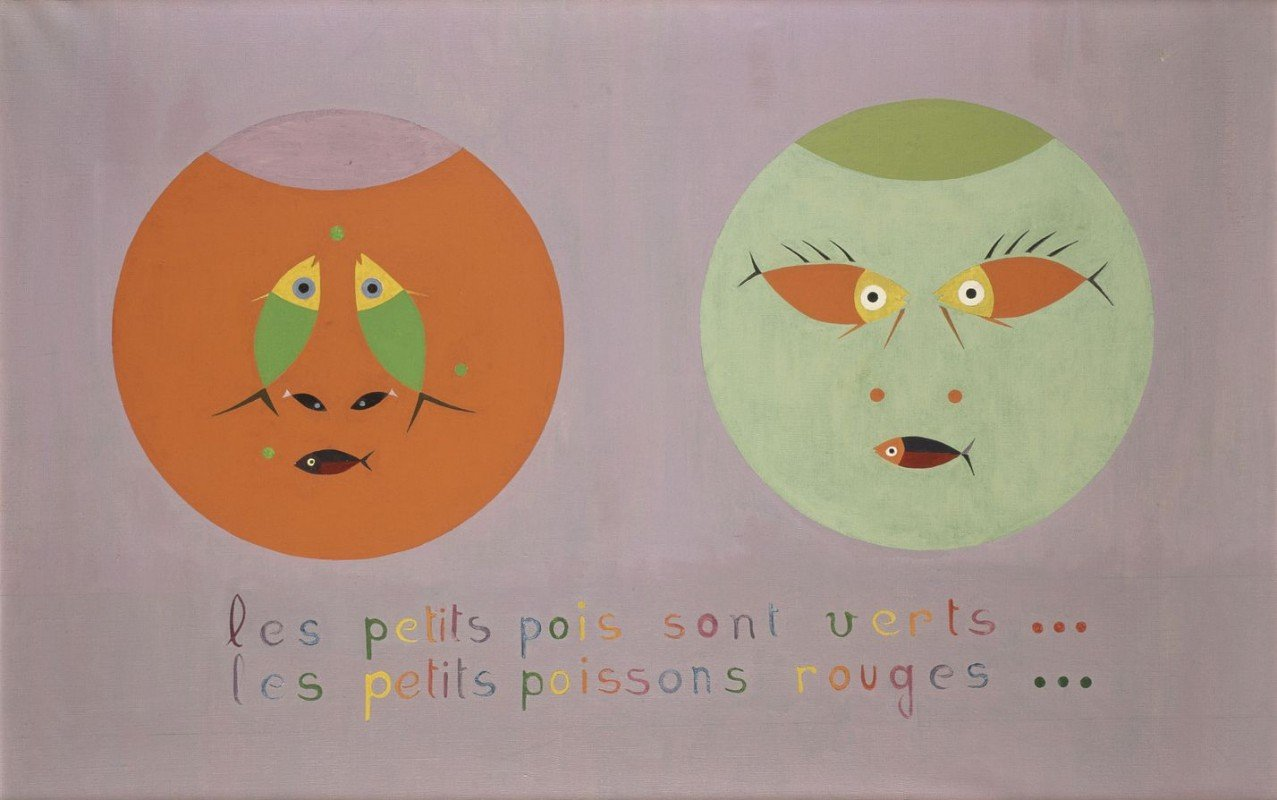
\includegraphics[width=1.1\textwidth]{les_petits_pois_sont_verts.jpeg}
\end{center}

~
\vfill
\thispagestyle{empty}
\setlength{\parindent}{0pt}
\setlength{\parskip}{\baselineskip}
Copyright \copyright\ \the\year\ \thanklessauthor

% \par\smallcaps{https://github.com/Naereen/Chasse-aux-tr-sors-au-Louvre-pour-mes-25-ans}

\par Cette œuvre est mise à disposition sous licence Attribution - Pas d'Utilisation Commerciale - Pas de Modification 4.0 International. Pour voir une copie de cette licence, visitez \url{http://creativecommons.org/licenses/by-nc-nd/4.0/} ou écrivez à Creative Commons, PO Box 1866, Mountain View, CA 94042, USA.\index{license}

\par\textit{Première édition, \monthyear}.
\end{fullwidth}

% r.5 contents
\setcounter{tocdepth}{2}

\begin{large}
  \tableofcontents
\end{large}

% \listoffigures
% \listoftables

% ---

% r.9 introduction
\cleardoublepage
\chapter{Introduction}

\vspace*{-30pt}

Chères amies et chers amis, merci d'avoir répondu présent !
%
Vous voilà réunis par \textbf{équipes de \intervalparequipe{} personnes},
et vous avez \textbf{\nbenigmes{}\footnote{C'est pas mes $26$ ans pour rien !} tâches à effectuer}.
%
Vous avez \textbf{1h30} : le musée évacue à \textbf{17h50} !
%
Rendez-vous à la sortie, \textbf{à 18h.}


\section*{Consignes}

L'ordre des énigmes est \emph{aléatoire}, elles ne sont triées ni par ordre chronologique, ni logique, ni spatial dans le musée, et n'ont aucune dépendance entres elles.
%
Toutes peuvent être résolues sans enfreindre le règlement intérieur du musée.
\textbf{Pas de triche} : n'utilisez pas vos téléphones intelligents pour chercher sur Internet !

Munissez vous d'un appareil photo ou de vos \emph{téléphones intelligents} : \textbf{toutes les énigmes demandent de trouver une œuvre et de la prendre en photo}\footnote{Sans flash ! Pas de retouchage des photos, non plus !}.
Économisez votre batterie et relayez vous.
%
Vous êtes réunis dans une équipe, pensez donc à mobilisez les idées\footnote{Je n'ai pas pu m'empêcher de glisser quelques calculs mathématiques… -- \emph{Lilian}} de tout le monde (et faites connaissance) !

L'objectif n'est pas d'être l'équipe la plus rapide mais celle qui répond à toutes les énigmes !
La coopération entre les autres équipes n'est pas recommandée.
La meilleure équipe recevra un prix à la fin de la visite !
%
Un dernier conseil : restez calmes et discrets… il ne faut pas que les vigiles détectent que vous vous êtes lancés dans une chasse aux trésors…


\section*{Bonne chance !}
Affûtez votre regard, aiguisez votre attention, entrez dans le Musée des Beaux Arts, et vous voilà près à affronter (pacifiquement) les autres équipes !



% r.10 all the enigmas
\cleardoublepage
\chapter{Énigmes}

\begin{fullwidth}
\input{all.tex}
\end{fullwidth}


% r.10 conclusion
\cleardoublepage
\chapter{À propos}

\section*{Un petit mot du créateur}

J'espère que ce livret et ce moment vont vous plaire !
Je me suis bien amusé à le concevoir, c'est déjà ça...

Si un problème survient, ou que vous bloquez sur une énigme, que vous pensez avoir besoin d'aide\footnote{Par exemple si vous pensez qu'une erreur s'est glissée dans ce document…}, n'hésitez pas à me contacter par téléphone ou m'appeler
\input{telephones.tex}.

J'ai hâte de vous retrouver à la sortie afin de décerner le \emph{prix de la meilleure équipe !}
Toutes les équipes auront une petite récompense, ne vous inquiétez pas…


\section*{Aspect ``technique'' \& remarques geek}
Ce document a été rédigé et compilé par mes soins, en sélectionnant \emph{aléatoirement} les \nbenigmes{} énigmes parmi une liste contenant \totalnbenigmes{} énigmes.
%
Chaque énigme a été rédigée comme un petit document Markdown\footnote{\url{DaringFireball.net/projects/markdown/}},
qui est ensuite compilé en \LaTeX{} par \texttt{pandoc}\footnote{\url{pandoc.org/}}.
%
Le document principal est un simple document \LaTeX,
utilisant le style épuré de Tufte-\LaTeX{}\footnote{\url{GitHub.com/Tufte-LaTeX/tufte-latex}}.
%
Les sources sont en accès libre\footnote{\url{frama.link/7Vzgqtgx}} et sous licence Creative Commons.

Ce recueil à été rédigé, imprimé et relié avec amour en janvier 2019.


\hfill{} -- \emph{Lilian Besson}.

\section*{Remarque importante}
\textbf{Aucun bénéfice financier n'a été ni ne sera tiré de ce document.}
C'est juste pour s'amuser !


\newpage
\blankpage

\end{document}
